\documentclass[11pt, a4paper]{article}

% Fonts and Encoding
\usepackage[utf8]{inputenc}
\usepackage[T1]{fontenc}
\usepackage{lmodern}
% Math and Symbols
\usepackage{amsmath, amssymb, amsthm, amsfonts, mathrsfs, mathtools}

% Layout and Geometry
\usepackage{geometry}
\geometry{a4paper, margin=1in}

% Formatting and Graphics
\usepackage{graphicx, xcolor, enumitem, booktabs, array, tabularx}

% TikZ for Illustrations
\usepackage{tikz}
\usetikzlibrary{arrows.meta, positioning, shapes.geometric, calc, backgrounds, matrix}

% Clickable Links and TOC
\usepackage{hyperref}
\hypersetup{
    colorlinks=true,
    linkcolor=blue,
    filecolor=magenta,      
    urlcolor=cyan,
    pdftitle={Advanced Mathematics Topic},
}

% Theorem Environments
\newtheorem{theorem}{Theorem}[section]
\newtheorem{lemma}[theorem]{Lemma}
\newtheorem{proposition}[theorem]{Proposition}
\newtheorem{corollary}[theorem]{Corollary}
\theoremstyle{definition}
\newtheorem{definition}{Definition}[section]
\newtheorem{axiom}{Axiom}[section]
\newtheorem{example}{Example}[section]
\theoremstyle{remark}
\newtheorem{remark}{Remark}[section]

% Custom Commands (Enforced standard notation)
\newcommand{\R}{\mathbb{R}}
\newcommand{\N}{\mathbb{N}}
\newcommand{\Z}{\mathbb{Z}}
\newcommand{\Q}{\mathbb{Q}}
\newcommand{\E}{\mathbb{E}}
\newcommand{\Prob}{\mathbb{P}}
\newcommand{\F}{\mathcal{F}}

\title{\textbf{Eigenvectors And Linear Transformations}}
\author{Tashfeen Omran}
\date{}

\begin{document}

\maketitle
\tableofcontents
\newpage

\section{Comprehensive Introduction, Context, And Prerequisites}

\subsection{Core Concepts}
The study of linear algebra frequently centers on understanding how linear transformations alter spaces. Let $V$ be a vector space and $T: V \to V$ be a linear transformation. An \textbf{eigenvector} of $T$ is a nonzero vector $\mathbf{x} \in V$ such that $T(\mathbf{x}) = \lambda \mathbf{x}$ for some scalar $\lambda$, which is called the \textbf{eigenvalue}. 

When $V$ is a finite-dimensional vector space, we can choose a basis $\mathcal{B} = \{\mathbf{b}_1, \dots, \mathbf{b}_n\}$. The transformation $T$ can then be represented by a matrix, known as the \textbf{$\mathcal{B}$-matrix for $T$}, denoted as $[T]_\mathcal{B}$. This matrix allows us to compute the action of $T$ using standard matrix multiplication on coordinate vectors:
\[
[T(\mathbf{x})]_\mathcal{B} = [T]_\mathcal{B} [\mathbf{x}]_\mathcal{B}
\]
If we are fortunate enough to find a basis $\mathcal{B}$ consisting entirely of eigenvectors of $T$, the resulting $\mathcal{B}$-matrix is \textbf{diagonal}. This drastically simplifies computations, as applying the transformation repeatedly (e.g., $T^k$) reduces to simply raising the diagonal entries to the $k$-th power.

\subsection{Intuition And Derivation}
Why do we care about changing bases and finding the $\mathcal{B}$-matrix? Imagine observing a complex physical system, like a spinning rigid body. From an arbitrary coordinate system, the equations of motion are dense and coupled (represented by a full matrix). However, if we align our axes with the object's natural axes of symmetry (the eigenvectors), the equations decouple. The transformation is now represented by a diagonal matrix. 

The formula for the $\mathcal{B}$-matrix is derived directly from the linearity of $T$ and the definition of coordinate vectors. If $\mathbf{x} = c_1\mathbf{b}_1 + \dots + c_n\mathbf{b}_n$, then:
\[
T(\mathbf{x}) = c_1T(\mathbf{b}_1) + \dots + c_nT(\mathbf{b}_n)
\]
Taking the coordinate mapping $[\cdot]_\mathcal{B}$ of both sides yields:
\[
[T(\mathbf{x})]_\mathcal{B} = c_1[T(\mathbf{b}_1)]_\mathcal{B} + \dots + c_n[T(\mathbf{b}_n)]_\mathcal{B} = \begin{bmatrix} [T(\mathbf{b}_1)]_\mathcal{B} & \dots & [T(\mathbf{b}_n)]_\mathcal{B} \end{bmatrix} \begin{bmatrix} c_1 \\ \vdots \\ c_n \end{bmatrix}
\]
Thus, the matrix $[T]_\mathcal{B}$ is simply the matrix whose columns are the $\mathcal{B}$-coordinate vectors of the images of the basis vectors.

\subsection{Historical Context And Motivation}
The concepts of eigenvalues and eigenvectors originated in the 18th century through the work of Leonhard Euler and Joseph-Louis Lagrange, who were studying the principal axes of rigid bodies and the stability of planetary orbits. In the 19th century, Augustin-Louis Cauchy formalized these ideas while studying quadratic forms and the stress tensor in elasticity. The motivation was fundamentally physical: mathematicians needed a way to find the "natural" coordinate system for a given linear operator where its behavior becomes as simple as possible (i.e., pure scaling).

\subsection{Key Formulas}
\renewcommand{\arraystretch}{1.5}
\begin{tabularx}{\textwidth}{l X}
\toprule
\textbf{Concept} & \textbf{Formula / Definition} \\
\midrule
$\mathcal{B}$-Matrix Definition & $\displaystyle [T]_\mathcal{B} = \left[ [T(\mathbf{b}_1)]_\mathcal{B} \quad [T(\mathbf{b}_2)]_\mathcal{B} \quad \dots \quad [T(\mathbf{b}_n)]_\mathcal{B} \right]$ \\
\addlinespace[4pt]
Coordinate Mapping Action & $\displaystyle [T(\mathbf{x})]_\mathcal{B} = [T]_\mathcal{B} [\mathbf{x}]_\mathcal{B}$ \\
\addlinespace[4pt]
Change of Basis for $\R^n$ & If $T(\mathbf{x}) = A\mathbf{x}$ and $P = [\mathbf{b}_1 \dots \mathbf{b}_n]$, then $\displaystyle [T]_\mathcal{B} = P^{-1}AP$ \\
\addlinespace[4pt]
Diagonalization & If $A = PDP^{-1}$, then the $\mathcal{B}$-matrix relative to the columns of $P$ is $D$. \\
\bottomrule
\end{tabularx}

\subsection{Prerequisites}
To master this topic, you must be proficient in:
\begin{itemize}
    \item \textbf{Vector Spaces and Bases:} Understanding linear independence, span, and how to find coordinate vectors $[\mathbf{x}]_\mathcal{B}$.
    \item \textbf{Matrix Operations:} Matrix multiplication, finding inverses ($P^{-1}$), and determinants.
    \item \textbf{Eigenvalues and Eigenvectors:} Solving the characteristic equation $\det(A - \lambda I) = 0$ and finding the null space $\text{Nul}(A - \lambda I)$.
\end{itemize}

\begin{figure}[h!]
\centering
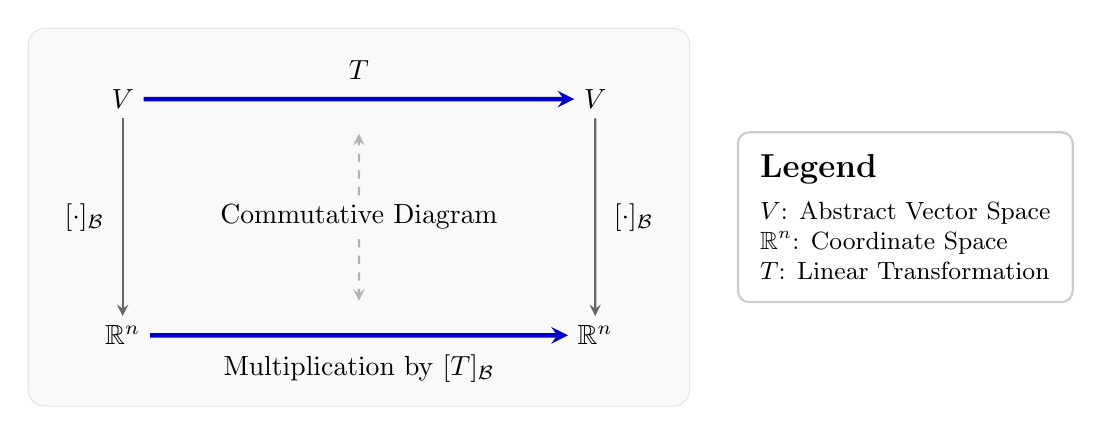
\begin{tikzpicture}[
    scale=1.5, % Globally expands coordinates for maximum breathing room
    >=stealth
]
    % 1. LAYER 1: Clean Background Canvas Block
    \draw[fill=gray!5, draw=gray!20, rounded corners=6pt] (-0.8, -1.6) rectangle (4.8, 1.6);

    % 2. LAYER 2: Structural Object Nodes
    \node (V1) at (0, 1) {$V$};
    \node (V2) at (4, 1) {$V$};
    \node (Rn1) at (0, -1) {$\mathbb{R}^n$};
    \node (Rn2) at (4, -1) {$\mathbb{R}^n$};

    % 3. LAYER 3: Morphism Mapping Arrows
    \draw[->, ultra thick, blue!80!black] (V1) -- (V2) node[midway, above=3pt, black] {$T$};
    \draw[->, ultra thick, blue!80!black] (Rn1) -- (Rn2) node[midway, below=3pt, black] {Multiplication by $[T]_\mathcal{B}$};
    \draw[->, thick, gray!80!black] (V1) -- (Rn1) node[midway, left=3pt, black] {$[\cdot]_\mathcal{B}$};
    \draw[->, thick, gray!80!black] (V2) -- (Rn2) node[midway, right=3pt, black] {$[\cdot]_\mathcal{B}$};

    % 4. LAYER 4: Central Commutativity Callouts
    \node (callout1) at (2, 0) {Commutative Diagram};
    \draw[->, thick, dashed, gray!60, shorten >=4pt] (callout1) -- (2, 0.8);
    \draw[->, thick, dashed, gray!60, shorten >=4pt] (callout1) -- (2, -0.8);

    % 5. LAYER 5: Dynamic Auto-Sizing Legend Node (Guaranteed Never to Overflow)
    \node[
        draw=gray!40,          % Border color
        fill=white,            % Background fill
        thick,                 % Border thickness
        rounded corners=4pt,   % Soft edges
        align=left,            % MANDATORY: Enables multiline text with \\
        inner sep=8pt,         % Padding inside the box around the text
        font=\small,           % Sets font size cleanly for all items
        anchor=west            % Anchors the left edge safely away from the diagram
    ] at (5.2, 0) {
        \textbf{\large Legend} \\[4pt]
        $V$: Abstract Vector Space \\
        $\mathbb{R}^n$: Coordinate Space \\
        $T$: Linear Transformation
    };

\end{tikzpicture}

\caption{The relationship between an abstract transformation $T$ and its matrix representation $[T]_\mathcal{B}$.}
\end{figure}

\newpage
\section{Detailed Homework Solutions}
\textit{Note: Following the strategic selection protocol, we have selected 12 highly representative problems that cover at least two of every distinct problem archetype found in the provided text.}

\subsection{Problem 1}
\textbf{Statement:} Let $\mathcal{B} = \{\mathbf{b}_1, \mathbf{b}_2, \mathbf{b}_3\}$ be a basis for a vector space $V$. Let $T: V \to V$ be a linear transformation with the property that $T(\mathbf{b}_1) = 3\mathbf{b}_1 - 5\mathbf{b}_2$, $T(\mathbf{b}_2) = -\mathbf{b}_1 + 6\mathbf{b}_2$, and $T(\mathbf{b}_3) = 4\mathbf{b}_2$. Find $[T]_\mathcal{B}$, the matrix for $T$ relative to $\mathcal{B}$.

\textbf{Solution:}
By definition, the $\mathcal{B}$-matrix for $T$ is constructed by finding the coordinate vectors of the images of the basis vectors and placing them as columns in a matrix:
\[
[T]_\mathcal{B} = \begin{bmatrix} [T(\mathbf{b}_1)]_\mathcal{B} & [T(\mathbf{b}_2)]_\mathcal{B} & [T(\mathbf{b}_3)]_\mathcal{B} \end{bmatrix}
\]
We extract the coordinates for each image relative to the basis $\mathcal{B}$:
\begin{align*}
    T(\mathbf{b}_1) &= 3\mathbf{b}_1 - 5\mathbf{b}_2 + 0\mathbf{b}_3 \quad \implies \quad [T(\mathbf{b}_1)]_\mathcal{B} = \begin{bmatrix} 3 \\ -5 \\ 0 \end{bmatrix} \\
    T(\mathbf{b}_2) &= -1\mathbf{b}_1 + 6\mathbf{b}_2 + 0\mathbf{b}_3 \quad \implies \quad [T(\mathbf{b}_2)]_\mathcal{B} = \begin{bmatrix} -1 \\ 6 \\ 0 \end{bmatrix} \\
    T(\mathbf{b}_3) &= 0\mathbf{b}_1 + 4\mathbf{b}_2 + 0\mathbf{b}_3 \quad \implies \quad [T(\mathbf{b}_3)]_\mathcal{B} = \begin{bmatrix} 0 \\ 4 \\ 0 \end{bmatrix}
\end{align*}
Concatenating these column vectors yields the final matrix:
\[
[T]_\mathcal{B} = \begin{bmatrix} 3 & -1 & 0 \\ -5 & 6 & 4 \\ 0 & 0 & 0 \end{bmatrix}
\]

\subsection{Problem 2}
\textbf{Statement:} Let $\mathcal{B} = \{\mathbf{b}_1, \mathbf{b}_2\}$ be a basis for a vector space $V$. Let $T: V \to V$ be a linear transformation with the property that $T(\mathbf{b}_1) = 7\mathbf{b}_1 + 4\mathbf{b}_2$ and $T(\mathbf{b}_2) = 6\mathbf{b}_1 - 5\mathbf{b}_2$. Find $[T]_\mathcal{B}$.

\textbf{Solution:}
Following the exact same logic as Problem 1, we find the coordinate vectors:
\begin{align*}
    [T(\mathbf{b}_1)]_\mathcal{B} &= \begin{bmatrix} 7 \\ 4 \end{bmatrix} \\
    [T(\mathbf{b}_2)]_\mathcal{B} &= \begin{bmatrix} 6 \\ -5 \end{bmatrix}
\end{align*}
Placing these as columns gives the final matrix:
\[
[T]_\mathcal{B} = \begin{bmatrix} 7 & 6 \\ 4 & -5 \end{bmatrix}
\]

\subsection{Problem 3}
\textbf{Statement:} Assume the mapping $T: \mathbb{P}_2 \to \mathbb{P}_2$ defined by $T(a_0 + a_1t + a_2t^2) = 2a_0 + (3a_1 + 4a_2)t + (5a_0 - 6a_2)t^2$ is linear. Find the matrix representation of $T$ relative to the basis $\mathcal{B} = \{1, t, t^2\}$.

\textbf{Solution:}
We must evaluate the transformation $T$ on each of the basis vectors in $\mathcal{B}$.
\begin{enumerate}
    \item For the first basis vector, $\mathbf{p}(t) = 1$. Here, $a_0 = 1, a_1 = 0, a_2 = 0$.
    \[
    T(1) = 2(1) + (0)t + (5(1) - 0)t^2 = 2 + 5t^2 \quad \implies \quad [T(1)]_\mathcal{B} = \begin{bmatrix} 2 \\ 0 \\ 5 \end{bmatrix}
    \]
    \item For the second basis vector, $\mathbf{p}(t) = t$. Here, $a_0 = 0, a_1 = 1, a_2 = 0$.
    \[
    T(t) = 0 + (3(1) + 0)t + 0t^2 = 3t \quad \implies \quad [T(t)]_\mathcal{B} = \begin{bmatrix} 0 \\ 3 \\ 0 \end{bmatrix}
    \]
    \item For the third basis vector, $\mathbf{p}(t) = t^2$. Here, $a_0 = 0, a_1 = 0, a_2 = 1$.
    \[
    T(t^2) = 0 + (0 + 4(1))t + (0 - 6(1))t^2 = 4t - 6t^2 \quad \implies \quad [T(t^2)]_\mathcal{B} = \begin{bmatrix} 0 \\ 4 \\ -6 \end{bmatrix}
    \]
\end{enumerate}
The matrix representation is formed by these columns:
\[
[T]_\mathcal{B} = \begin{bmatrix} 2 & 0 & 0 \\ 0 & 3 & 4 \\ 5 & 0 & -6 \end{bmatrix}
\]

\subsection{Problem 4}
\textbf{Statement:} Define $T: \mathbb{P}_2 \to \mathbb{P}_2$ by $T(\mathbf{p}) = \mathbf{p}(0) - \mathbf{p}(1)t + \mathbf{p}(2)t^2$.
a. Show that $T$ is a linear transformation.
b. Find $T(\mathbf{p})$ when $\mathbf{p}(t) = -2 + t$. Is $\mathbf{p}$ an eigenvector of $T$?
c. Find the matrix for $T$ relative to the basis $\{1, t, t^2\}$.

\textbf{Solution:}
\textbf{Part (a):} To show $T$ is linear, we must show $T(c\mathbf{p} + \mathbf{q}) = cT(\mathbf{p}) + T(\mathbf{q})$ for any scalar $c$ and polynomials $\mathbf{p}, \mathbf{q} \in \mathbb{P}_2$.
\begin{align*}
    T(c\mathbf{p} + \mathbf{q}) &= (c\mathbf{p} + \mathbf{q})(0) - (c\mathbf{p} + \mathbf{q})(1)t + (c\mathbf{p} + \mathbf{q})(2)t^2 \\
    &= (c\mathbf{p}(0) + \mathbf{q}(0)) - (c\mathbf{p}(1) + \mathbf{q}(1))t + (c\mathbf{p}(2) + \mathbf{q}(2))t^2 \\
    &= c\left( \mathbf{p}(0) - \mathbf{p}(1)t + \mathbf{p}(2)t^2 \right) + \left( \mathbf{q}(0) - \mathbf{q}(1)t + \mathbf{q}(2)t^2 \right) \\
    &= cT(\mathbf{p}) + T(\mathbf{q})
\end{align*}
Thus, $T$ is a linear transformation.

\textbf{Part (b):} Let $\mathbf{p}(t) = -2 + t$. We evaluate $\mathbf{p}$ at $0, 1,$ and $2$:
\[
\mathbf{p}(0) = -2, \quad \mathbf{p}(1) = -1, \quad \mathbf{p}(2) = 0
\]
Applying the transformation:
\[
T(\mathbf{p}) = (-2) - (-1)t + (0)t^2 = -2 + t
\]
Since $T(\mathbf{p}) = 1 \cdot \mathbf{p}(t)$, and $\mathbf{p}(t)$ is not the zero polynomial, $\mathbf{p}$ is indeed an eigenvector of $T$ corresponding to the eigenvalue $\lambda = 1$.

\textbf{Part (c):} We evaluate $T$ on the standard basis $\mathcal{B} = \{1, t, t^2\}$.
\begin{align*}
    \mathbf{b}_1(t) = 1 &\implies \mathbf{b}_1(0)=1, \mathbf{b}_1(1)=1, \mathbf{b}_1(2)=1 \implies T(1) = 1 - t + t^2 \implies \begin{bmatrix} 1 \\ -1 \\ 1 \end{bmatrix} \\
    \mathbf{b}_2(t) = t &\implies \mathbf{b}_2(0)=0, \mathbf{b}_2(1)=1, \mathbf{b}_2(2)=2 \implies T(t) = 0 - t + 2t^2 \implies \begin{bmatrix} 0 \\ -1 \\ 2 \end{bmatrix} \\
    \mathbf{b}_3(t) = t^2 &\implies \mathbf{b}_3(0)=0, \mathbf{b}_3(1)=1, \mathbf{b}_3(2)=4 \implies T(t^2) = 0 - t + 4t^2 \implies \begin{bmatrix} 0 \\ -1 \\ 4 \end{bmatrix}
\end{align*}
The matrix representation is:
\[
[T]_\mathcal{B} = \begin{bmatrix} 1 & 0 & 0 \\ -1 & -1 & -1 \\ 1 & 2 & 4 \end{bmatrix}
\]

\subsection{Problem 7}
\textbf{Statement:} Find the $\mathcal{B}$-matrix for the transformation $\mathbf{x} \mapsto A\mathbf{x}$, when $\mathcal{B} = \{\mathbf{b}_1, \mathbf{b}_2\}$.
\[
A = \begin{bmatrix} 4 & 9 \\ 1 & 4 \end{bmatrix}, \quad \mathbf{b}_1 = \begin{bmatrix} 3 \\ -1 \end{bmatrix}, \quad \mathbf{b}_2 = \begin{bmatrix} 1 \\ 1 \end{bmatrix}
\]

\textbf{Solution:}
The change of coordinates matrix from $\mathcal{B}$ to the standard basis is $P = \begin{bmatrix} \mathbf{b}_1 & \mathbf{b}_2 \end{bmatrix} = \begin{bmatrix} 3 & 1 \\ -1 & 1 \end{bmatrix}$.
The $\mathcal{B}$-matrix is given by the formula $[T]_\mathcal{B} = P^{-1}AP$.
First, we find $P^{-1}$:
\[
\det(P) = (3)(1) - (1)(-1) = 4 \quad \implies \quad P^{-1} = \frac{1}{4} \begin{bmatrix} 1 & -1 \\ 1 & 3 \end{bmatrix}
\]
Next, we compute $AP$:
\[
AP = \begin{bmatrix} 4 & 9 \\ 1 & 4 \end{bmatrix} \begin{bmatrix} 3 & 1 \\ -1 & 1 \end{bmatrix} = \begin{bmatrix} (12 - 9) & (4 + 9) \\ (3 - 4) & (1 + 4) \end{bmatrix} = \begin{bmatrix} 3 & 13 \\ -1 & 5 \end{bmatrix}
\]
Finally, we compute $P^{-1}(AP)$:
\[
[T]_\mathcal{B} = \frac{1}{4} \begin{bmatrix} 1 & -1 \\ 1 & 3 \end{bmatrix} \begin{bmatrix} 3 & 13 \\ -1 & 5 \end{bmatrix} = \frac{1}{4} \begin{bmatrix} (3 + 1) & (13 - 5) \\ (3 - 3) & (13 + 15) \end{bmatrix} = \frac{1}{4} \begin{bmatrix} 4 & 8 \\ 0 & 28 \end{bmatrix} = \begin{bmatrix} 1 & 2 \\ 0 & 7 \end{bmatrix}
\]
Final Answer: $[T]_\mathcal{B} = \begin{bmatrix} 1 & 2 \\ 0 & 7 \end{bmatrix}$.

\subsection{Problem 8}
\textbf{Statement:} Find the $\mathcal{B}$-matrix for the transformation $\mathbf{x} \mapsto A\mathbf{x}$, when $\mathcal{B} = \{\mathbf{b}_1, \mathbf{b}_2\}$.
\[
A = \begin{bmatrix} -1 & 4 \\ -2 & 3 \end{bmatrix}, \quad \mathbf{b}_1 = \begin{bmatrix} 3 \\ 2 \end{bmatrix}, \quad \mathbf{b}_2 = \begin{bmatrix} -1 \\ 1 \end{bmatrix}
\]

\textbf{Solution:}
We construct $P = \begin{bmatrix} 3 & -1 \\ 2 & 1 \end{bmatrix}$.
The determinant is $\det(P) = (3)(1) - (-1)(2) = 5$.
\[
P^{-1} = \frac{1}{5} \begin{bmatrix} 1 & 1 \\ -2 & 3 \end{bmatrix}
\]
Compute $AP$:
\[
AP = \begin{bmatrix} -1 & 4 \\ -2 & 3 \end{bmatrix} \begin{bmatrix} 3 & -1 \\ 2 & 1 \end{bmatrix} = \begin{bmatrix} (-3 + 8) & (1 + 4) \\ (-6 + 6) & (2 + 3) \end{bmatrix} = \begin{bmatrix} 5 & 5 \\ 0 & 5 \end{bmatrix}
\]
Compute $P^{-1}(AP)$:
\[
[T]_\mathcal{B} = \frac{1}{5} \begin{bmatrix} 1 & 1 \\ -2 & 3 \end{bmatrix} \begin{bmatrix} 5 & 5 \\ 0 & 5 \end{bmatrix} = \frac{1}{5} \begin{bmatrix} 5 & 10 \\ -10 & 5 \end{bmatrix} = \begin{bmatrix} 1 & 2 \\ -2 & 1 \end{bmatrix}
\]
Final Answer: $[T]_\mathcal{B} = \begin{bmatrix} 1 & 2 \\ -2 & 1 \end{bmatrix}$.

\subsection{Problem 9}
\textbf{Statement:} Define $T: \R^2 \to \R^2$ by $T(\mathbf{x}) = A\mathbf{x}$. Find a basis $\mathcal{B}$ for $\R^2$ with the property that $[T]_\mathcal{B}$ is diagonal.
\[
A = \begin{bmatrix} 0 & 1 \\ -3 & 4 \end{bmatrix}
\]

\textbf{Solution:}
To find a basis that diagonalizes the transformation, we must find the eigenvectors of $A$.
First, find the eigenvalues by solving $\det(A - \lambda I) = 0$:
\[
\det \begin{bmatrix} -\lambda & 1 \\ -3 & 4 - \lambda \end{bmatrix} = -\lambda(4 - \lambda) - (-3)(1) = \lambda^2 - 4\lambda + 3 = 0
\]
Factoring yields $(\lambda - 1)(\lambda - 3) = 0$, so the eigenvalues are $\lambda_1 = 1$ and $\lambda_2 = 3$.

Next, find the corresponding eigenvectors:
For $\lambda_1 = 1$:
\[
A - I = \begin{bmatrix} -1 & 1 \\ -3 & 3 \end{bmatrix} \sim \begin{bmatrix} 1 & -1 \\ 0 & 0 \end{bmatrix} \quad \implies \quad x_1 - x_2 = 0 \quad \implies \quad \mathbf{v}_1 = \begin{bmatrix} 1 \\ 1 \end{bmatrix}
\]
For $\lambda_2 = 3$:
\[
A - 3I = \begin{bmatrix} -3 & 1 \\ -3 & 1 \end{bmatrix} \sim \begin{bmatrix} 3 & -1 \\ 0 & 0 \end{bmatrix} \quad \implies \quad 3x_1 - x_2 = 0 \quad \implies \quad \mathbf{v}_2 = \begin{bmatrix} 1 \\ 3 \end{bmatrix}
\]
The basis $\mathcal{B}$ consists of these eigenvectors:
\[
\mathcal{B} = \left\{ \begin{bmatrix} 1 \\ 1 \end{bmatrix}, \begin{bmatrix} 1 \\ 3 \end{bmatrix} \right\}
\]

\subsection{Problem 10}
\textbf{Statement:} Define $T: \R^2 \to \R^2$ by $T(\mathbf{x}) = A\mathbf{x}$. Find a basis $\mathcal{B}$ for $\R^2$ with the property that $[T]_\mathcal{B}$ is diagonal.
\[
A = \begin{bmatrix} 5 & -3 \\ -7 & 1 \end{bmatrix}
\]

\textbf{Solution:}
Find the eigenvalues:
\[
\det(A - \lambda I) = \det \begin{bmatrix} 5 - \lambda & -3 \\ -7 & 1 - \lambda \end{bmatrix} = (5 - \lambda)(1 - \lambda) - 21 = \lambda^2 - 6\lambda + 5 - 21 = \lambda^2 - 6\lambda - 16 = 0
\]
Factoring yields $(\lambda - 8)(\lambda + 2) = 0$, so $\lambda_1 = 8$ and $\lambda_2 = -2$.

Find the eigenvectors:
For $\lambda_1 = 8$:
\[
A - 8I = \begin{bmatrix} -3 & -3 \\ -7 & -7 \end{bmatrix} \sim \begin{bmatrix} 1 & 1 \\ 0 & 0 \end{bmatrix} \quad \implies \quad x_1 + x_2 = 0 \quad \implies \quad \mathbf{v}_1 = \begin{bmatrix} 1 \\ -1 \end{bmatrix}
\]
For $\lambda_2 = -2$:
\[
A + 2I = \begin{bmatrix} 7 & -3 \\ -7 & 3 \end{bmatrix} \sim \begin{bmatrix} 7 & -3 \\ 0 & 0 \end{bmatrix} \quad \implies \quad 7x_1 - 3x_2 = 0 \quad \implies \quad \mathbf{v}_2 = \begin{bmatrix} 3 \\ 7 \end{bmatrix}
\]
The basis $\mathcal{B}$ is:
\[
\mathcal{B} = \left\{ \begin{bmatrix} 1 \\ -1 \end{bmatrix}, \begin{bmatrix} 3 \\ 7 \end{bmatrix} \right\}
\]

\subsection{Problem 17}
\textbf{Statement:} True or False: Similar matrices have the same eigenvalues. Justify your answer.

\textbf{Solution:}
\textbf{True.} Let $A$ and $B$ be similar matrices. By definition, there exists an invertible matrix $P$ such that $A = PBP^{-1}$. We examine the characteristic polynomial of $A$:
\begin{align*}
    \det(A - \lambda I) &= \det(PBP^{-1} - \lambda I) \\
    &= \det(PBP^{-1} - \lambda PIP^{-1}) \\
    &= \det(P(B - \lambda I)P^{-1}) \\
    &= \det(P) \det(B - \lambda I) \det(P^{-1})
\end{align*}
Since $\det(P)\det(P^{-1}) = \det(PP^{-1}) = \det(I) = 1$, we have:
\[
\det(A - \lambda I) = \det(B - \lambda I)
\]
Because their characteristic polynomials are identical, their roots (the eigenvalues) must be exactly the same.

\subsection{Problem 18}
\textbf{Statement:} True or False: Similar matrices have the same eigenvectors. Justify your answer.

\textbf{Solution:}
\textbf{False.} While similar matrices share eigenvalues, their eigenvectors are generally different. Suppose $A = PBP^{-1}$ and $\mathbf{v}$ is an eigenvector of $B$ corresponding to $\lambda$. Then $B\mathbf{v} = \lambda \mathbf{v}$.
Let us see how $A$ acts on the vector $P\mathbf{v}$:
\[
A(P\mathbf{v}) = (PBP^{-1})(P\mathbf{v}) = PB(P^{-1}P)\mathbf{v} = PB\mathbf{v} = P(\lambda \mathbf{v}) = \lambda(P\mathbf{v})
\]
This shows that if $\mathbf{v}$ is an eigenvector of $B$, then $P\mathbf{v}$ is the corresponding eigenvector of $A$. Unless $P = I$ (which means $A=B$), the eigenvectors $\mathbf{v}$ and $P\mathbf{v}$ are distinct.

\subsection{Problem 21}
\textbf{Statement:} If $A$ is invertible and similar to $B$, then $B$ is invertible and $A^{-1}$ is similar to $B^{-1}$. Explain why $B$ is invertible. Then find an invertible $Q$ such that $Q^{-1}A^{-1}Q = B^{-1}$.

\textbf{Solution:}
Since $A$ is similar to $B$, there exists an invertible matrix $P$ such that $A = PBP^{-1}$.
First, we show $B$ is invertible. Taking the determinant of both sides:
\[
\det(A) = \det(PBP^{-1}) = \det(B)
\]
Since $A$ is invertible, $\det(A) \neq 0$. Therefore, $\det(B) \neq 0$, which proves $B$ is invertible.

Next, we find the similarity transformation for the inverses. Starting with $A = PBP^{-1}$, we take the inverse of both sides:
\begin{align*}
    A^{-1} &= (PBP^{-1})^{-1} \\
    A^{-1} &= (P^{-1})^{-1} B^{-1} P^{-1} \quad \text{(using the property } (XYZ)^{-1} = Z^{-1}Y^{-1}X^{-1} \text{)} \\
    A^{-1} &= P B^{-1} P^{-1}
\end{align*}
To match the form $Q^{-1}A^{-1}Q = B^{-1}$, we multiply on the left by $P^{-1}$ and on the right by $P$:
\[
P^{-1} A^{-1} P = B^{-1}
\]
Thus, the required matrix is $Q = P$.

\subsection{Problem 22}
\textbf{Statement:} If $A$ is similar to $B$, then $A^2$ is similar to $B^2$.

\textbf{Solution:}
Since $A$ is similar to $B$, there exists an invertible matrix $P$ such that $A = PBP^{-1}$.
We compute $A^2$:
\begin{align*}
    A^2 &= A \cdot A \\
    &= (PBP^{-1})(PBP^{-1}) \\
    &= PB(P^{-1}P)BP^{-1} \\
    &= PB(I)BP^{-1} \\
    &= PB^2P^{-1}
\end{align*}
This equation, $A^2 = P(B^2)P^{-1}$, is precisely the definition of $A^2$ being similar to $B^2$, using the exact same change-of-basis matrix $P$.

\newpage
\section{In-Depth Analysis of Problems and Techniques}

\subsection{A) Problem Types and General Approach}
The homework problems can be categorized into five distinct archetypes:

1. \textbf{Abstract Basis Mapping (Problems 1, 2):}
   \textit{Approach:} These problems test the fundamental definition of the $\mathcal{B}$-matrix. You are given the images of the basis vectors directly. The strategy is simply to extract the coefficients of these images relative to the basis $\mathcal{B}$ and arrange them as column vectors to form $[T]_\mathcal{B}$.

2. \textbf{Polynomial Transformations (Problems 3, 4):}
   \textit{Approach:} These problems require mapping the abstract space of polynomials $\mathbb{P}_2$ to $\R^3$. The strategy is to evaluate the transformation on the standard polynomial basis $\{1, t, t^2\}$, collect the resulting polynomials, and extract their coefficients to form the columns of the matrix.

3. \textbf{Change of Basis for $\R^n$ (Problems 7, 8):}
   \textit{Approach:} You are given a standard matrix $A$ and a new basis $\mathcal{B}$. The strategy relies on the formula $[T]_\mathcal{B} = P^{-1}AP$, where $P$ is the matrix whose columns are the vectors in $\mathcal{B}$.

4. \textbf{Diagonalization (Problems 9, 10):}
   \textit{Approach:} The goal is to find a basis that makes the transformation matrix diagonal. The strategy is to solve the eigenvalue problem for $A$. The roots of the characteristic polynomial give the eigenvalues, and the null spaces of $(A - \lambda I)$ give the eigenvectors. These eigenvectors form the required basis $\mathcal{B}$.

5. \textbf{Theoretical Proofs on Similarity (Problems 17, 18, 21, 22):}
   \textit{Approach:} These problems require algebraic manipulation of the similarity definition $A = PBP^{-1}$. The strategy involves applying properties of determinants, inverses, and matrix multiplication to show that properties (like eigenvalues or invertibility) are preserved under similarity transformations.

\subsection{B) Key Algebraic and Calculus Manipulations}
\begin{itemize}
    \item \textbf{Coordinate Extraction by Inspection:} In Problem 1, converting $T(\mathbf{b}_1) = 3\mathbf{b}_1 - 5\mathbf{b}_2$ into the vector $[3, -5, 0]^T$ requires recognizing that the coefficients of the basis vectors directly form the components of the coordinate vector.
    \item \textbf{The $P^{-1}AP$ Computation:} In Problems 7 and 8, computing $P^{-1}AP$ efficiently is crucial. A common trick is to compute $AP$ first, and then multiply by $P^{-1}$ on the left. This avoids dealing with fractions from $P^{-1}$ until the very last step.
    \item \textbf{Characteristic Polynomial Factoring:} In Problems 9 and 10, finding eigenvalues requires expanding $\det(A - \lambda I)$ into a quadratic equation $\lambda^2 - \text{tr}(A)\lambda + \det(A) = 0$ and factoring it.
    \item \textbf{Null Space via Row Reduction:} To find eigenvectors, we must solve $(A - \lambda I)\mathbf{x} = \mathbf{0}$. Because $\lambda$ is an eigenvalue, the rows of $A - \lambda I$ will always be linearly dependent. The trick is to only look at the first non-zero row to deduce the relationship between $x_1$ and $x_2$ (e.g., $x_1 - x_2 = 0 \implies \mathbf{x} = [1, 1]^T$).
    \item \textbf{Telescoping Matrix Multiplication:} In Problem 22, proving $A^2 = PB^2P^{-1}$ relies on the "telescoping" nature of the inner terms: $(P^{-1}P) = I$. This trick generalizes to $A^k = PB^kP^{-1}$.
\end{itemize}

\newpage
\section{"Cheatsheet" and Tips for Success}

\renewcommand{\arraystretch}{1.5}
\begin{tabularx}{\textwidth}{l X}
\toprule
\textbf{Category} & \textbf{Details} \\
\midrule
\textbf{Core Formula} & $\displaystyle [T]_\mathcal{B} = \left[ [T(\mathbf{b}_1)]_\mathcal{B} \quad \dots \quad [T(\mathbf{b}_n)]_\mathcal{B} \right]$ \\
\addlinespace[4pt]
\textbf{Similarity} & $A$ and $B$ are similar if there exists invertible $P$ such that $A = PBP^{-1}$. \\
\addlinespace[4pt]
\textbf{Diagonalization} & If $A = PDP^{-1}$, the columns of $P$ are eigenvectors, and $D$ contains eigenvalues. \\
\addlinespace[4pt]
\textbf{2x2 Inverse Trick} & $\displaystyle \begin{bmatrix} a & b \\ c & d \end{bmatrix}^{-1} = \frac{1}{ad-bc} \begin{bmatrix} d & -b \\ -c & a \end{bmatrix}$ \\
\addlinespace[4pt]
\textbf{Eigenvalue Shortcut} & For a $2 \times 2$ matrix, $\lambda^2 - \text{tr}(A)\lambda + \det(A) = 0$. \\
\bottomrule
\end{tabularx}

\vspace{1em}
\textbf{Common Pitfalls and Traps:}
\begin{itemize}
    \item \textbf{Reversing $P$ and $P^{-1}$:} When computing the $\mathcal{B}$-matrix for $A$, the formula is $P^{-1}AP$, not $PAP^{-1}$. Remember that $P$ takes you from $\mathcal{B}$-coordinates to standard coordinates, so to go $\mathcal{B} \to \mathcal{B}$, you must first go $\mathcal{B} \to \text{Standard}$ (via $P$), apply $A$, and then go $\text{Standard} \to \mathcal{B}$ (via $P^{-1}$).
    \item \textbf{Forgetting the Zero Vector Rule:} An eigenvector \textit{must} be non-zero by definition. If you solve $(A - \lambda I)\mathbf{x} = \mathbf{0}$ and only get the trivial solution $\mathbf{x} = \mathbf{0}$, you have made an arithmetic error in finding your eigenvalues.
    \item \textbf{Assuming Similar Matrices have the Same Eigenvectors:} As proven in Problem 18, they share eigenvalues, but their eigenvectors are transformed by $P$.
\end{itemize}

\section{Conceptual Synthesis and The "Big Picture"}

\subsection{A) Thematic Connections}
The central theme of this topic is \textbf{Isomorphism and Representation}. In mathematics, we often deal with abstract spaces (like the space of polynomials $\mathbb{P}_2$ or the space of continuous signals). By choosing a basis, we create an isomorphism (a structural mapping) between these abstract spaces and the concrete, familiar space of $\R^n$. The $\mathcal{B}$-matrix is the ultimate manifestation of this theme: it allows us to perform abstract linear transformations using standard, algorithmic matrix multiplication. This mirrors the concept of a "coordinate system" in geometry, where abstract points are represented by tuples of numbers.

\subsection{B) Forward and Backward Links}
\textbf{Backward Links:} This topic heavily relies on the foundational concepts of linear independence, span, and basis. It is the logical culmination of the eigenvalue/eigenvector chapter, providing the geometric \textit{reason} why we care about diagonalizing matrices.

\textbf{Forward Links:} Understanding matrix representations relative to different bases is the bedrock for advanced linear algebra and functional analysis. 
\begin{itemize}
    \item \textbf{Singular Value Decomposition (SVD):} Later, you will learn that even if a matrix isn't square or diagonalizable, you can find two different bases (one for the domain, one for the codomain) that make the transformation matrix diagonal.
    \item \textbf{Quantum Mechanics:} In quantum theory, observables are linear operators. Changing the basis corresponds to changing the observable being measured (e.g., switching from position space to momentum space via the Fourier transform).
\end{itemize}

\newpage
\section{Abstract Real-World Modeling (AI, ML, \& Quant Finance)}

\subsection{A) Concrete Scenarios}
\begin{enumerate}
    \item \textbf{Quantitative Finance (Principal Component Analysis on Yield Curves):} Interest rates for different maturities (1-year, 5-year, 10-year bonds) move together but not perfectly. Quants use the covariance matrix of these rate changes. By finding the eigenvectors of this matrix (a change of basis), they identify the "Principal Components" (usually interpreted as parallel shift, steepening, and curvature of the yield curve). This diagonalizes the risk, allowing traders to hedge independent risk factors.
    \item \textbf{Machine Learning (Markov Chains and PageRank):} The Google PageRank algorithm models the internet as a massive transition matrix $M$. The "importance" of a webpage is the steady-state vector of this system, which is precisely the eigenvector corresponding to the eigenvalue $\lambda = 1$.
    \item \textbf{Generative AI (Latent Space Disentanglement):} In Variational Autoencoders (VAEs), the goal is to map complex data (like images) into a lower-dimensional latent space. Ideally, we want the covariance matrix of this latent space to be diagonal, meaning the features (like "smile" or "glasses" on a face) are mathematically disentangled and can be controlled independently.
\end{enumerate}

\subsection{B) Model Problem Setup: PCA in Quantitative Finance}
Let us rigorously model the yield curve risk using Principal Component Analysis. 

\textbf{State Space and Random Variables:}
Let $\mathbf{r}_t \in \R^n$ be a random vector representing the daily changes in interest rates for $n$ different maturities at time $t$. We assume $\mathbf{r}_t$ is drawn from a multivariate normal distribution with mean $\mathbf{0}$ and an $n \times n$ covariance matrix $\Sigma$:
\[
\mathbf{r}_t \sim \mathcal{N}(\mathbf{0}, \Sigma) \quad \text{where} \quad \Sigma = \E[\mathbf{r}_t \mathbf{r}_t^T]
\]
Because $\Sigma$ is a symmetric, positive semi-definite matrix, the Spectral Theorem guarantees that it is orthogonally diagonalizable. 

\textbf{The Optimization Problem:}
We seek a new orthonormal basis $\mathcal{B} = \{\mathbf{v}_1, \dots, \mathbf{v}_n\}$ such that the variance of the data projected onto these vectors is maximized sequentially. This is equivalent to finding the matrix $P = [\mathbf{v}_1 \dots \mathbf{v}_n]$ such that the $\mathcal{B}$-matrix representation of the covariance is diagonal:
\[
[T]_\mathcal{B} = P^T \Sigma P = \Lambda = \begin{bmatrix} \lambda_1 & 0 & \dots & 0 \\ 0 & \lambda_2 & \dots & 0 \\ \vdots & \vdots & \ddots & \vdots \\ 0 & 0 & \dots & \lambda_n \end{bmatrix}
\]
where $\lambda_1 \geq \lambda_2 \geq \dots \geq \lambda_n \geq 0$. The eigenvectors $\mathbf{v}_i$ represent the independent risk factors (the "eigen-portfolios"), and the eigenvalues $\lambda_i$ represent the variance explained by each factor.

\begin{figure}[h!]
\centering
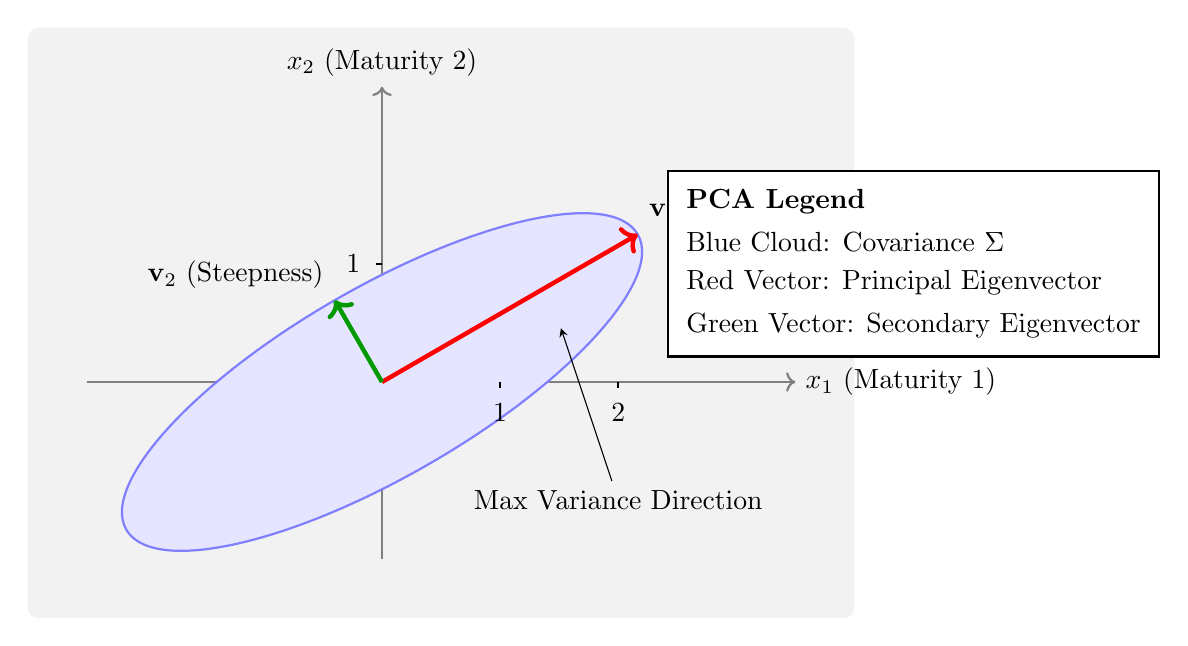
\begin{tikzpicture}[scale=1.5]
    % Background Layer
    \begin{scope}[on background layer]
        \fill[gray!10, rounded corners] (-3, -2) rectangle (4, 3);
    \end{scope}

    % Axes
    \draw[->, thick, gray] (-2.5, 0) -- (3.5, 0) node[right, text=black] {$x_1$ (Maturity 1)};
    \draw[->, thick, gray] (0, -1.5) -- (0, 2.5) node[above, text=black] {$x_2$ (Maturity 2)};

    % Data Cloud (Ellipse)
    \draw[thick, blue!50, fill=blue!10, rotate around={30:(0,0)}] (0,0) ellipse (2.5 and 0.8);

    % Eigenvectors
    \draw[->, ultra thick, red] (0,0) -- (2.165, 1.25) node[above right, text=black] {$\displaystyle \mathbf{v}_1$ (Shift)};
    \draw[->, ultra thick, green!60!black] (0,0) -- (-0.4, 0.692) node[above left, text=black] {$\displaystyle \mathbf{v}_2$ (Steepness)};

    % Explicit Tick Marks
    \draw[thick] (1, 0) -- (1, -0.05) node[below=2pt] {$1$};
    \draw[thick] (2, 0) -- (2, -0.05) node[below=2pt] {$2$};
    \draw[thick] (0, 1) -- (-0.05, 1) node[left=2pt] {$1$};

    % Callout
    \node (callout) at (2, -1) {Max Variance Direction};
    \draw[->, >=stealth, shorten >=2pt] (callout) -- (1.5, 0.5);

    % Matrix Legend
    \matrix [matrix of nodes, draw, thick, fill=white, nodes={anchor=west}] at (4.5, 1) {
        \textbf{PCA Legend} \\
        Blue Cloud: Covariance $\Sigma$ \\
        Red Vector: Principal Eigenvector \\
        Green Vector: Secondary Eigenvector \\
    };
\end{tikzpicture}
\caption{Diagonalizing the covariance matrix $\Sigma$ aligns the coordinate axes with the eigenvectors, decoupling the financial risk factors.}
\end{figure}

\newpage
\section{Common Variations and Untested Concepts}

\subsection{The Defective Matrix and Jordan Canonical Form}
The provided homework focuses heavily on matrices that \textit{can} be diagonalized. A critical missing concept is what happens when a matrix does not have enough linearly independent eigenvectors to form a basis for $\R^n$. Such a matrix is called \textbf{defective}.

When a matrix is defective, it cannot be diagonalized ($A \neq PDP^{-1}$). Instead, the best we can do is find a basis that puts the matrix into \textbf{Jordan Canonical Form}, which is "almost" diagonal, having 1s on the superdiagonal above the repeated eigenvalues.

\textbf{Example Problem:} Let $A = \begin{bmatrix} 4 & 1 \\ -1 & 2 \end{bmatrix}$. Show that $A$ is defective, and find the $\mathcal{B}$-matrix for $T(\mathbf{x}) = A\mathbf{x}$ using a basis consisting of an eigenvector and a generalized eigenvector.

\textbf{Solution:}
1. Find eigenvalues: $\det(A - \lambda I) = (4-\lambda)(2-\lambda) + 1 = \lambda^2 - 6\lambda + 9 = (\lambda - 3)^2 = 0$. So $\lambda = 3$ (algebraic multiplicity 2).
2. Find eigenvectors: 
\[
A - 3I = \begin{bmatrix} 1 & 1 \\ -1 & -1 \end{bmatrix} \sim \begin{bmatrix} 1 & 1 \\ 0 & 0 \end{bmatrix} \implies \mathbf{v}_1 = \begin{bmatrix} 1 \\ -1 \end{bmatrix}
\]
There is only one linearly independent eigenvector. The geometric multiplicity is 1, which is less than the algebraic multiplicity (2). Thus, $A$ is defective.
3. Find a generalized eigenvector $\mathbf{v}_2$ such that $(A - 3I)\mathbf{v}_2 = \mathbf{v}_1$:
\[
\begin{bmatrix} 1 & 1 \\ -1 & -1 \end{bmatrix} \begin{bmatrix} x_1 \\ x_2 \end{bmatrix} = \begin{bmatrix} 1 \\ -1 \end{bmatrix} \implies x_1 + x_2 = 1 \implies \text{Let } \mathbf{v}_2 = \begin{bmatrix} 1 \\ 0 \end{bmatrix}
\]
4. Form the basis $\mathcal{B} = \{\mathbf{v}_1, \mathbf{v}_2\}$ and matrix $P = \begin{bmatrix} 1 & 1 \\ -1 & 0 \end{bmatrix}$.
5. Compute $[T]_\mathcal{B} = P^{-1}AP$:
\[
P^{-1} = \begin{bmatrix} 0 & -1 \\ 1 & 1 \end{bmatrix} \implies [T]_\mathcal{B} = \begin{bmatrix} 0 & -1 \\ 1 & 1 \end{bmatrix} \begin{bmatrix} 4 & 1 \\ -1 & 2 \end{bmatrix} \begin{bmatrix} 1 & 1 \\ -1 & 0 \end{bmatrix} = \begin{bmatrix} 3 & 1 \\ 0 & 3 \end{bmatrix}
\]
This upper triangular matrix is the Jordan block for $\lambda = 3$.

\newpage
\section{Advanced Diagnostic Testing: "Find the Flaw"}

Below are five problems with complete solutions. However, each solution contains a single, subtle, yet critical flaw. Your task as the grader is to find the error, explain why it is wrong in one sentence, and provide the correct final solution.

\subsection{Flawed Problem 1}
\textbf{Problem:} Let $T: \R^2 \to \R^2$ be defined by $T(\mathbf{x}) = A\mathbf{x}$ where $A = \begin{bmatrix} 2 & 1 \\ 0 & 3 \end{bmatrix}$. Let $\mathcal{B} = \left\{ \begin{bmatrix} 1 \\ 1 \end{bmatrix}, \begin{bmatrix} 0 \\ 1 \end{bmatrix} \right\}$. Find $[T]_\mathcal{B}$.
\textbf{Flawed Solution:}
We compute the images of the basis vectors under $A$:
$T(\mathbf{b}_1) = \begin{bmatrix} 2 & 1 \\ 0 & 3 \end{bmatrix} \begin{bmatrix} 1 \\ 1 \end{bmatrix} = \begin{bmatrix} 3 \\ 3 \end{bmatrix}$.
$T(\mathbf{b}_2) = \begin{bmatrix} 2 & 1 \\ 0 & 3 \end{bmatrix} \begin{bmatrix} 0 \\ 1 \end{bmatrix} = \begin{bmatrix} 1 \\ 3 \end{bmatrix}$.
We place these images as the rows of the matrix to find $[T]_\mathcal{B}$:
$[T]_\mathcal{B} = \begin{bmatrix} 3 & 3 \\ 1 & 3 \end{bmatrix}$.

\subsection{Flawed Problem 2}
\textbf{Problem:} Let $T: \mathbb{P}_1 \to \mathbb{P}_1$ be defined by $T(a + bt) = (a+b) + (2b)t$. Find the matrix for $T$ relative to $\mathcal{B} = \{1, t\}$.
\textbf{Flawed Solution:}
We evaluate $T$ on the basis vectors.
For $\mathbf{b}_1 = 1$, $a=1, b=0$. $T(1) = 1 + 0t$. The coordinate vector is $[1, 0]^T$.
For $\mathbf{b}_2 = t$, $a=0, b=1$. $T(t) = 1 + 2t$. The coordinate vector is $[1, 2]^T$.
Therefore, $[T]_\mathcal{B} = \begin{bmatrix} 1 & 1 \\ 0 & 2 \end{bmatrix}$.
Since this matrix is upper triangular, the eigenvalues are 1 and 2. The eigenvector for $\lambda=2$ is found by solving $([T]_\mathcal{B} - 2I)\mathbf{x} = \mathbf{0} \implies \begin{bmatrix} -1 & 1 \\ 0 & 0 \end{bmatrix}\mathbf{x} = \mathbf{0} \implies \mathbf{x} = \begin{bmatrix} 1 \\ 1 \end{bmatrix}$.
Thus, the eigenvector in $\mathbb{P}_1$ is $\mathbf{p}(t) = 1 + 1$.

\subsection{Flawed Problem 3}
\textbf{Problem:} Find the $\mathcal{B}$-matrix for $A = \begin{bmatrix} 1 & 2 \\ 3 & 4 \end{bmatrix}$ relative to $\mathcal{B} = \left\{ \begin{bmatrix} 1 \\ 0 \end{bmatrix}, \begin{bmatrix} 1 \\ 1 \end{bmatrix} \right\}$.
\textbf{Flawed Solution:}
Let $P = \begin{bmatrix} 1 & 1 \\ 0 & 1 \end{bmatrix}$. The formula for the $\mathcal{B}$-matrix is $[T]_\mathcal{B} = PAP^{-1}$.
$P^{-1} = \begin{bmatrix} 1 & -1 \\ 0 & 1 \end{bmatrix}$.
$[T]_\mathcal{B} = \begin{bmatrix} 1 & 1 \\ 0 & 1 \end{bmatrix} \begin{bmatrix} 1 & 2 \\ 3 & 4 \end{bmatrix} \begin{bmatrix} 1 & -1 \\ 0 & 1 \end{bmatrix} = \begin{bmatrix} 4 & 6 \\ 3 & 4 \end{bmatrix} \begin{bmatrix} 1 & -1 \\ 0 & 1 \end{bmatrix} = \begin{bmatrix} 4 & 2 \\ 3 & 1 \end{bmatrix}$.

\subsection{Flawed Problem 4}
\textbf{Problem:} Find the eigenvalues of $A = \begin{bmatrix} 2 & 4 \\ 1 & -1 \end{bmatrix}$.
\textbf{Flawed Solution:}
We solve $\det(A - \lambda I) = 0$.
$\det \begin{bmatrix} 2-\lambda & 4 \\ 1 & -1-\lambda \end{bmatrix} = (2-\lambda)(-1-\lambda) - 4 = -2 - 2\lambda + \lambda + \lambda^2 - 4 = \lambda^2 - \lambda - 6 = 0$.
Factoring gives $(\lambda - 3)(\lambda + 2) = 0$.
Therefore, the eigenvalues are $\lambda = -3$ and $\lambda = 2$.

\subsection{Flawed Problem 5}
\textbf{Problem:} True or False: If $A$ is diagonalizable, then any matrix $B$ similar to $A$ is also diagonalizable.
\textbf{Flawed Solution:}
False. If $A$ is diagonalizable, $A = PDP^{-1}$. If $B$ is similar to $A$, then $B = QAQ^{-1}$ for some invertible $Q$. Substituting $A$, we get $B = Q(PDP^{-1})Q^{-1}$. Because the matrices $Q$ and $P$ do not necessarily commute, we cannot simplify this to the form $B = M D M^{-1}$. Therefore, $B$ might not be diagonalizable.

\vspace{2em}
\hrule
\vspace{1em}
\textbf{Grader Answer Key (For Self-Correction):}
\begin{itemize}
    \item \textbf{Flaw 1:} The student placed the images $T(\mathbf{b}_i)$ as rows instead of columns, and failed to convert them into $\mathcal{B}$-coordinates first. Correct $[T]_\mathcal{B} = \begin{bmatrix} 3 & 1 \\ 0 & 2 \end{bmatrix}$.
    \item \textbf{Flaw 2:} The student correctly found the coordinate vector $[1, 1]^T$, but incorrectly translated it back to $\mathbb{P}_1$ as $1+1$ instead of $1(1) + 1(t) = 1+t$.
    \item \textbf{Flaw 3:} The student used the incorrect formula $PAP^{-1}$ instead of the correct change-of-basis formula $P^{-1}AP$. Correct $[T]_\mathcal{B} = \begin{bmatrix} -2 & -3 \\ 3 & 7 \end{bmatrix}$.
    \item \textbf{Flaw 4:} The student factored $\lambda^2 - \lambda - 6 = (\lambda - 3)(\lambda + 2) = 0$ but incorrectly extracted the roots as $-3$ and $2$ instead of $3$ and $-2$.
    \item \textbf{Flaw 5:} The student claimed $Q(PDP^{-1})Q^{-1}$ cannot be written as $MDM^{-1}$, but by associativity, $B = (QP)D(QP)^{-1}$, so $B$ is indeed diagonalizable with $M = QP$. The statement is True.
\end{itemize}

\end{document}